\section{Personagens}

\subsection{Introdução}
O jogo apresentará duas classes de dificuldades ao personagem principal 
(ou jogador): de percurso e de inimigos. As dificuldades de percurso serão 
aquelas apresentadas pelo ambiente e que exigirá a habilidade de locomoção 
do personagem, tal como salto ou desvio de obstáculos. As dificuldades 
de inimigos serão aquelas que exigirão a habilidade de ataque e defesa 
do personagem quando em confronto com um inimigo.

Nas seções a seguir são apresentadas as formas de controle dos estados 
do personagem principal, os inimigos e suas respectivas características 
e, por fim, o cenário e seus desafios.

\subsection{Estados do Personagem Principal}
Na primeira fase do jogo, haverá duas barras para que o jogador possa 
controlar os estados do per-sonagem principal, ou seja, a condição física 
dele: a barra de vida e a barra de energia.
 
\subsubsection{Barra de Vida}
A barra de vida exibe o nível de vitalidade do personagem principal. 
A Figura 1 apresenta um esboço desta barra, que começa completa, com
100 pontos percentuais. São dois os fatores que influenciarão no 
decaimento do nível: ataques sofridos e barra de energia vazia. Os ataques 
sofridos condizem com os ata-ques dos animais que o personagem encontrará
nos cenários da primeira fase. O valor que será decremen-tado da barra de 
vida dependerá da força de ataque do animal em específico. Sobre a barra de 
energia vazia e a forma de recuperação da força vital do personagem, estas
são tratadas na subseção a seguir.

\begin{figure}[!ht]
 \centering
 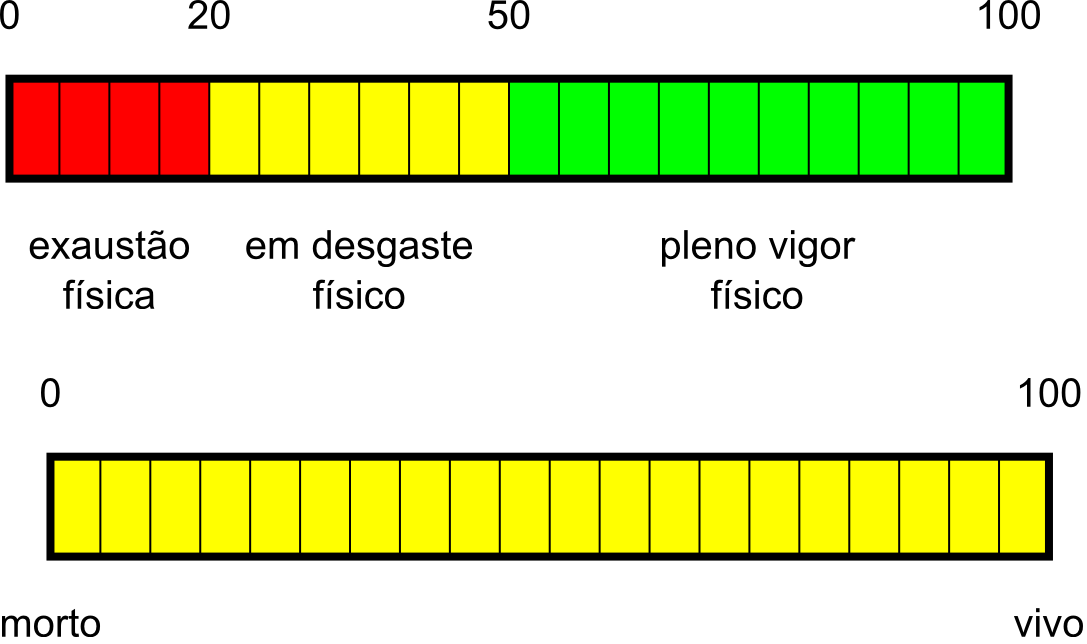
\includegraphics[scale=3]{BarraDeEnergia.png}
 \caption{Esboço das barras de vida (acima) e energia (abaixo).}
 \label{img:energia}
\end{figure}

\subsubsection{Barra de Energia}
A barra de energia exibe o nível de resistência física do personagem principal, 
ou seja, a capacidade dele para desenvolver um esforço físico. A Figura 1 apresenta 
um esboço desta barra, que inicia cheia. No intervalo de 50 a 100, destacado em 
verde, o personagem estará em pleno vigor físico. Ele conseguirá correr e pular 
alto ou longas distâncias. No intervalo de 20 a 50, destacado em amarelo, o 
personagem começará a sofrer um desgaste físico. Ele passará a correr cada vez 
mais lento e a saltar alturas e distâncias cada vez menores até chegar à exaustão 
física – a função para controle da capacidade de esforço físico do persona-gem é 
apresentada no Gráfico 1. No intervalo de 0 a 20, o personagem já não conseguirá 
mais correr e nem pular, apenas andar.

\begin{figure}[!ht]
 \centering
 \includegraphics[scale=2.5]{VelocidadeDeDeslocamentoEPulo.png}
 \caption{Relação entre a capacidade de esforço físico e a energia do personagem.}
 \label{img:velocidade}
\end{figure}

Os fatores que influenciarão no decaimento do nível de resistência física 
do personagem são: deslocamento, pulo e golpe. No deslocamento, o nível de 
energia deverá reduzir linearmente em função da distância percorrida pelo 
personagem. A cada pulo ou golpe realizado pelo personagem será decrementado 
ao nível de energia 1 e 1/2 ponto percentual, respectivamente. Se a barra de 
energia estiver vazia, estes fatores deverão interferir, na mesma proporção, 
no nível de vitalidade do personagem. Para elevar ambos os níveis de 
resistência física e de vitalidade, o personagem deverá matar e, em 
seguida, se alimentar dos animais que ele encontrará pelo caminho. Cada 
animal tem o seu valor energético específico.

\subsection{Personagens}
Na primeira fase, os inimigos do personagem principal serão os animais da floresta. 
Haverá cinco espécies de animais: cobra, urso, abelha, jacaré e tigre. Cada espécie 
terá suas características específicas. Estas são apresentadas na Tabela 1, em que K 
é um valor constante e p.p. é a abreviação de pontos percentuais.

\begin{figure}[!ht]
 \centering
 \includegraphics[scale=1]{tabela.png}
 \caption{}
 \label{img:tabela}
\end{figure}

\subsection{Personagem principal}
\subsubsection{Descrição física e psicológica}
Medrash é o personagem principal, o qual será controlado pelo jogador. Ele
 possui cerca de 20 anos de idade, 1,65 m de altura e 70 Kg. Com um corpo
 magro, mas com músculos definidos, é muito forte, sendo tipicamente um
 caçador.

Ele é um caçador da tribo Ari e marido de Sora. Medrash tem sua esposa e
 amigos sequestrados no inicio do jogo e seu objetivo principal é 
resgatalos.

Medrash enfrenta diferentes inimigos ao longo do jogo. É corajoso,
 determinado e não desiste de resgatar seus companheiros mesmo diante de
 todos os perigos enfrentados ao longo do caminho. É um homem bom e astuto,
 oferecendo ajuda a uma tribo aliada e juntando forças com os mesmos a fim
 de enfrentar a poderosa tribo Luskan.

\subsubsection{Concepção artística}
O Modelo base de Medrash está mostrado na figura \ref{img:medrash}

\begin{figure}[!ht]
 \centering
 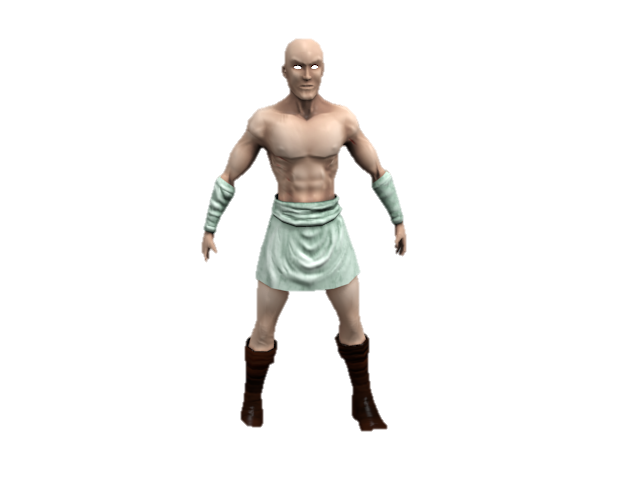
\includegraphics[scale=0.5]{Imagens/medrash01.png}
 \caption{Medrash}
 \label{img:medrash}
\end{figure}


\subsubsection{Armas do personagem principal}
\begin{itemize}
\item {\bf Porrete}
O porrete é a arma inicial de Medrash. Simples, rápida e fácil de usar,
 esta arma pode ser utilizada para atacar a maior parte dos inimigos da
 primeira fase.

A Figura \ref{img:porrete} mostra uma concepção artística desta arma.

IMAGEM (porrete)

\item {\bf Lança}
A lança é a segunda arma de Medrash, encontrada ainda na primeira fase,
 podendo ser adquirida de um guerreiro morto. Ela apresenta um grande poder
 de perfuração, sendo assim, mais eficiente que o porrete para caçar
 tigres.

A concepção artistica da lança está na figura \ref{img:lanca}.

IMAGEM (lanca)

\item {\bf Machado}
Adquirido na segunda parte da fase 2, é uma das melhores armas de Medrash
 para lutar contra a furiosa tribo Luskan. (Detalhar mais sobre a arma).

O conceito artístico do machado pode ser encontrado na figura 
\ref{img:machado}.

IMAGEM (machado)

\end{itemize}

\subsection{Personagens Secundários}
\subsubsection{Sora}
Sora é mulher de Medrash, vivendo pacificamente na tribo Ari. Sequestrada
 por Balazar para ser escravizada, precisa da ajuda de Medrash para poder
 ser livre novamente.
\begin{itemize}
\item {\bf Descrição física}
Com aproximadamente 18 anos, com 1.55 m de altura e 50 Kg, 
\item {\bf Concepção artística}
O modelo de Sora está demonstrado na figura \ref{img:sora}.

IMAGEM (sora)

As animações para este personagem são:
\begin{itemize}
\item Ficar parada (gritando, movimentando-se);
\item Corre.
\end{itemize}
\end{itemize}

\subsubsection{Gardain}
Um dos principais guerreiros da tribo Ari, a tribo de Medrash, e o único
 sobrevivente do ataque da tribo Luskan. Ao retornar de sua caçada, Medrash
 vê sua tribo totalmente devastada, restando apenas Gardain como
 sobrevivente. Mesmo estando muito machucado, Gardain conta a Medrash que
 os Luskans fizeram todos da tribo prisioneiros, inclusive sua amada Sora. 
\begin{itemize}
\item {\bf Descrição Física}
Gardain é um guerreiro forte, porém, devido a batalha com a tribo Luskan
 encontra-se esgotado e com diversos ferimentos pelo corpo.
\item {\bf Concepção Artística}
O modelo que servirá como base para a criação de Gardain é apresentado na
 Figura \ref{img:gardain}. Alterações de vestimenta e maiores detalhes
 serão acrescentados para a concepção do personagem.

IMAGEM (gardain)

\end{itemize}
\subsubsection{Rangrim}
Rangrim é o líder da tribo dos Mara-kai. Ao chegar na tribo, Medrash
 encontra-o ferido após ataque da tribo Luskan. Rangrim informa Medrash de
 que os Luskan pretendem atacar a tribo aliada Akanul, a maior e mais
 importante da região. Experiente e sábio, Rangrim conhece bem os caminhos
 e perigos da região, e indica a Medrash um atalho através das montanhas
 Kabalus, o que permitirá que Medrash chegue a tribo Akanul muito antes dos
 Luskans.
\begin{itemize}
\item {\bf Descrição Física}
Ancião, Rangrim é magro e de baixa estatura. Cabelos e barba branca,
 Rangrim anda de maneira curvada devido a idade avançada.
\item {\bf Concepção Artística}
O ancião apresentado na Figura \ref{rangrim} será utilizado para a criação
 do personagem Rangrim. Alterações de vestimenta serão realizadas para que
 se adeque ao período do jogo.

IMAGEM (rangrim)

\end{itemize}
\subsection{Inimigos}
\subsubsection{Cobra}
Não é um inimigo direito de Medrash, só ataca quando se sente ameaçada. A
 cobra é a segunda menor criatura do jogo atrás apenas da abelha. Ela
 patrulha uma determinada área rastejando e, caso o personagem principal se
 aproxime, esta fica enrolada em posição de ataque efetuando bote em forma
 de mordida caso a distância diminua. Se o personagem principal se
 distanciar a cobra volta a patrulhar a área. A cobra está presente apenas
 na primeira fase do jogo.
\begin{itemize}
\item {\bf Descrição Física}
Como mencionado, a cobra é um dos menores inimigos de Medrash. Medindo
 cerca de 80 cm, tem aparência realista e possui presas afiadas para o seu
 único ataque, a mordida. A tabela 1 apresenta as principais
 características da cobra, onde K é um valor constante e p.p. é a
 abreviação para pontos percentuais.

TABELA

\item {\bf Concepção Artística}
O modelo da cobra está mostrado abaixo:

IMAGEM

As animações para este personagem são:
\begin{itemize}
\item Rastejar;
\item Enrolar para o ataque;
\item Bote/Ataque;
\end{itemize}
\end{itemize}

\subsubsection{Urso}
O urso é o maior inimigo de Medrash e está presente somente na primeira
 fase do jogo. Se Medrash se aproximar muito dele, o urso se defenderá,
 perseguindo Medrash. Ao alcança-lo, o urso o ataca. O distanciamento de
 Medrash faz o urso esquecê-lo, voltando a patrulhar a região do mapa.
\begin{itemize}
\item {\bf Descrição física}
O urso pesa aproximadamente 400 Kg, tendo até 4 m de altura quando em
 posição bípede. Ele é muito robusto e apresenta pelagem marrom.

TABELA

\item {\bf Concepção Artística}
O modelo definido para o urso está mostrado na Figura \ref{img:urso}.

IMAGEM (urso)

As animações que o urso deverá ter são:
\begin{itemize}
\item Andar;
\item Correr;
\item Ficar sobre as patas traseiras;
\item Abraçar e morder Medrash.
\end{itemize}
\end{itemize}

\subsubsection{Jacaré}
O jacaré é um inimigo natural também encontrado na primeira fase do jogo.
 Vive ao redor de um rio, o qual Medrash é obrigado a atravessar para ir de
 um cenário à outro. O jacaré basicamente fica parado à margem do rio, e/ou
 nadando nele. Da mesma forma que a cobra, o jacaré só ataca se Medrash
 chegar muito próximo dele, nesse caso ele começa a persegui-lo tanto
 dentro como fora d'água. Se Medrash estiver muito perto do jacaré, este
 irá atacá-lo, ou seja, irá abocanhar Medrash. Caso Medrash se distancie o
 jacaré volta à sua posição inicial.
\begin{itemize}
\item {\bf Descrição Física}
O jacaré também possui aparência realista, com cerca de 2m de comprimento e
 pesando 80 Kg. Possui dentes afiados e maior agilidade dentro da água.
 Fora dela se torna muito mais lento, porém possui o mesmo poder de ataque.
 A tabela 2 descreve as principais características do jacaré.

\item {\bf Concepção Artística}
Ainda não foi definido um modelo específico que representará o jacaré,
 porém, o modelo da Figura \ref{img:jacare} servirá como base para concepção do
 personagem.

IMAGEM (jacare)

Animações que o jacaré deverá ter:
\begin{itemize}
\item Andar;
\item Nadar;
\item Abocanhar/Morder;
\end{itemize}
\end{itemize}